%%%% début de la page
\sndEnTeteDeux

%%
\nomPrenomClasse


%%%% titre
\numeroActivite{4}
\titreActivite{Modéliser une action}


%%%% objectifs
\vspace{-10pt}
\begin{objectifs}
  \item Comprendre la notion de force
  \item Connaître la force d'interaction gravitationnelle
  \item Comprendre le lien entre la force d'interaction gravitationnelle et le poids
\end{objectifs}


%%%% evaluation
\begin{tableauCompetences}
  \centering Communication (COM) &
  Travailler en groupe, échanger entre élèves.
  & & & &
\end{tableauCompetences}


%%%%
\titreSection{Système et référentiel}

%%%%
\vspace{-10pt}
\begin{doc}{Satellite Hubble}
  \begin{wrapfigure}{l}{0.4\linewidth}
    \image{1}{images/mouvements/hubble}
  \end{wrapfigure}
  
  Le satellite Hubble est un satellite de masse $m_S = 1,\!1 \times 10^4 \unit{kg}$ conçu par la NASA avec une  participation de l'Agence spatiale européenne, l'ESA.
  
  Ce satellite est opérationnel depuis 1990 et tourne autour de la Terre en 96 min.
  Vu depuis le centre de la Terre, il a un mouvement circulaire uniforme autour de la Terre, à une altitude $h = 590 \unit{km}$.
  
  Ce satellite contient un télescope qui permet d’observer les étoiles et objets de l’univers depuis l’espace !
\end{doc}

%%
\begin{doc}{Force et action mécanique}
  \chevron Un corps exerce une \important{action mécanique} sur le système étudié si \reponseLigne
  \reponse{1}
  
  Pour modéliser une action mécanique, on utilise le concept de \important{force}.
  
  \begin{encart}
    La force exercée par un corps $A$ sur un corps $B$ est représentée par un vecteur \vFAsurB}.
    Ce vecteur possède les caractéristiques suivantes :
    \begin{listePoints}
      \item Une \important{norme} notée \FAsurB, qui s'exprime en \dotfill
      \item Une \important{direction} et un \important{sens} qui dépendent de la situation.
      \item Un \important{point d'application} : le centre du système $B$.
    \end{listePoints}
  \end{encart}
\end{doc}

%%
\newpage
\bgin{doc}{Force d'interaction gravitationnelle}
  \chevron Tous les corps qui possèdent une masse s’attirent entre eux : c’est l’attraction gravitationnelle.

  \begin{encart}
    On modélise l'attraction gravitationnelle exercée par le corps $A$ sur le corps $B$ par une force représentée par un vecteur $\vvFAsurB$ :
    
    \begin{wrapfigure}[2]{r}{0.4\linewidth}
      \vspace*{-105pt}
      \begin{tikzpicture}
        % corps A et B
        \tkzCercle{0}{0}{gray!50!white}{20}
        \tkzLabel{-1.2}{0}{$m_A$}
        \tkzCercle{4}{2}{gray!50!white}{20}
        \tkzLabel{2.8}{2}{$m_B$}
        \tkzPointLabel{0}{0}{$A$}
        \tkzPointLabel{4}{2}{$B$}
        % force et distance
        \tkzVecteur{4}{2}{-1.5}{-0.75}{$\vvFAsurB$}{left}
        \tkzVecteur{0.5}{-1}{4}{2}{\phantom{G}$d$}{right}
      \end{tikzpicture}
    \end{wrapfigure}
    
    \begin{listePoints}
      \item \important{Point d'application} : centre du corps $B$
      \item \important{Direction} : la droite $AB$.
      \item \important{Sens} : de $B$ vers $A$ (force attractive).
      \item \important{Norme} : $\FAsurB = \ldots\ldots\ldots$
    \end{listePoints}
      
    Dans la formule de la norme de la force, les masses s'expriment en kilogramme (kg), la distance en mètre (m) et la \important{constante universelle de gravitation} $G$ en newton mètre carrée par kilogramme carrée ($\!\!\unit{N \cdot m^2 \cdot kg^{-2}}$). Sa valeur (à connaître) est 
    \begin{equation*}
      G = \ldots\ldots\ldots\ldots
      %6,67 \times 10^{-11}
      \unit{N \cdot m^2 \cdot kg^{-2}}
    \end{equation*}
  \end{encart}
\end{doc}

%%%%
\question{
  Compléter les documents \ref{doc:force_action} et \ref{doc:gravitation}.
}{0}

\question{
  Donner trois exemples d'actions mécaniques qu'on peut rencontrer dans la vie quotidienne.
}{5}

\question{
  Quelle différence remarquez-vous entre ces actions de la vie quotidienne et l'action exercée par la Terre sur le satellite Hubble ?
}{3}

\question{
  Sur le schéma ci-dessous, représenter la force d’interaction gravitationnelle #»F T /S exercée par la Terre T sur le satellite Hubble S.
  La Terre est assimilée à une boule de rayon RT = 6,37 × 103 km et de masse MT = 5,97 × 1024 kg.
}{0}

\question{
   En utilisant le document 3, donner la relation qui relie la norme de la force FT/S et la masse du satellite mS, la masse de la Terre MT, la constante G et la distance d.
}{2}